\documentclass[11pt]{article}

% ─── Core packages ───
\usepackage[utf8]{inputenc}
\usepackage[T1]{fontenc}
\usepackage{times}
\usepackage[margin=1in]{geometry}
\usepackage{amsmath,amssymb,amsfonts}
\usepackage{graphicx}
\usepackage{booktabs}
\usepackage{multirow}
\usepackage{enumitem}
\usepackage{hyperref}
\usepackage{xcolor}
\usepackage{algorithm}
\usepackage{algorithmic}
\usepackage{caption}
\usepackage{subcaption}
\usepackage{float}
\usepackage{natbib}
\usepackage{microtype}

\hypersetup{
  colorlinks=true,
  linkcolor=blue!70!black,
  citecolor=blue!70!black,
  urlcolor=blue!70!black
}

% ─── Custom commands ───
\newcommand{\method}{\textsc{IWEUP v2}}
\newcommand{\Loss}{\mathcal{L}}

\title{Selective Machine Unlearning via Adaptive Confidence Reduction:\\
A Unified Framework for Class-Level and Sample-Level Data Removal}

\author{
  Author Name\textsuperscript{1} \\
  \textsuperscript{1}International Institute of Information Technology, Hyderabad \\
  \texttt{author@iiit.ac.in}
}

\date{}

\begin{document}
\maketitle

% ══════════════════════════════════════════════════════════════
% ABSTRACT
% ══════════════════════════════════════════════════════════════
\begin{abstract}
The proliferation of privacy regulations such as the EU's General Data Protection Regulation (GDPR) and the ``Right to be Forgotten'' has created an urgent need for mechanisms that can selectively remove the influence of specific training data from deployed machine learning models without the prohibitive cost of full retraining.
We present \method{}, a unified machine unlearning framework capable of operating at both \textit{class-level} and \textit{sample-level} forgetting granularities, coupled with a novel \textbf{information-theoretic auditing framework} based on Partial Information Decomposition (PID) that rigorously certifies whether unlearning has truly removed information.
Our approach employs a hybrid loss function combining Maximum Entropy Regularization with Adaptive Confidence Reduction, while our auditing framework uses the \textbf{Residual Knowledge metric ($I_\cap$)} to quantify information that persists after unlearning.
We conduct extensive experiments on CIFAR-10 and CIFAR-100 using ResNet-18, benchmarking against seven baselines across three random seeds.
For class-level forgetting, \method{} achieves a \textbf{0.000 MIA score} on both datasets, matching the retrained model while being up to \textbf{10$\times$ faster}.
Our information decomposition audit reveals that \method{} achieves an $I_\cap$ of \textbf{0.122 $\pm$ 0.016 bits}---closest to the retrained gold standard (0.076 $\pm$ 0.009)---while traditional metrics like Forget Accuracy fail to distinguish methods with similar residual information.
A stress-test protocol further demonstrates that all audited methods show consistent behavior across easy-to-forget and hard-to-forget samples, with \method{} achieving $I_\cap = 0.000$ across all difficulty splits.
Code and demo are publicly available.
\end{abstract}

\noindent\textbf{Keywords:} Machine Unlearning, Privacy, GDPR, Membership Inference Attack, Deep Learning, Selective Forgetting

% ══════════════════════════════════════════════════════════════
% 1. INTRODUCTION
% ══════════════════════════════════════════════════════════════
\section{Introduction}
\label{sec:introduction}

Deep neural networks achieve state-of-the-art performance across numerous tasks but are known to memorize individual training examples~\citep{carlini2022membership, feldman2020does}. This memorization creates a fundamental tension with emerging privacy legislation: once a model is trained, removing the influence of specific data points is non-trivial. The naive solution---retraining the model from scratch on the remaining data---is computationally prohibitive, especially for large-scale deployments where deletion requests may arrive continuously.

\textbf{Machine Unlearning}~\citep{bourtoule2021machine, cao2015towards} addresses this challenge by modifying a trained model's parameters so that it behaves as though certain data was never part of the training set. An effective unlearning algorithm must satisfy three desiderata:
\begin{enumerate}[leftmargin=*]
    \item \textbf{Efficacy:} The model should not retain information about the forgotten data.
    \item \textbf{Utility:} The model's performance on retained and unseen data should be preserved.
    \item \textbf{Efficiency:} The unlearning process should be significantly faster than full retraining.
\end{enumerate}

Existing approaches often excel at one criterion while failing at others. Gradient Ascent~\citep{thudi2022unrolling} can erase information but catastrophically degrades utility. Fine-tuning on retained data preserves utility but fails to erase deep memorization. SCRUB~\citep{kurmanji2023towards} balances these via knowledge distillation but introduces significant computational overhead.

Furthermore, most existing methods are designed and evaluated for \textit{class-level} forgetting---removing an entire class of data---which is a coarse-grained task. The more practically relevant scenario of \textit{sample-level} forgetting (e.g., removing one user's contributions, typically $<$5\% of training data) remains underexplored and poses unique challenges: the model must ``forget'' specific samples without altering its decision boundaries for the classes those samples belong to.

\subsection{Contributions}
We make the following contributions:
\begin{enumerate}[leftmargin=*]
    \item We propose \method{}, a unified unlearning framework that automatically adapts its forgetting strategy based on the granularity of the deletion request (class vs.\ sample).
    \item We introduce a novel three-component sample-level loss function combining \textit{Adaptive Confidence Reduction}, \textit{Anti-Memorization Penalty}, and \textit{MIA-Fooling Regularization}.
    \item We adapt the Partial Information Decomposition (PID) framework~\citep{gutknecht2021bits} and RINE estimator~\citep{mazzetto2025auditing} to build a \textbf{representation-level auditing framework} for certifying unlearning in vision models.
    \item We introduce a \textbf{stress-test protocol} that constructs difficulty-ranked forget sets (easy, hard, random) using per-sample Residual Knowledge ($I_\cap$) scores and evaluates method robustness across these splits.
    \item We conduct comprehensive multi-seed experiments on CIFAR-10 and CIFAR-100, benchmarking against seven baselines using both traditional metrics and our $I_\cap$-based audit.
\end{enumerate}

% ══════════════════════════════════════════════════════════════
% 2. LITERATURE REVIEW
% ══════════════════════════════════════════════════════════════
\section{Related Work}
\label{sec:related}

\paragraph{Exact Unlearning.}
\citet{bourtoule2021machine} introduced SISA (Sharded, Isolated, Sliced, and Aggregated Training), which partitions data into shards so that retraining is limited to the affected shard. While providing exact guarantees, SISA incurs significant overhead at inference time and does not scale to modern architectures trained on monolithic datasets.

\paragraph{Approximate Unlearning.}
\citet{golatkar2020eternal} proposed using Fisher Information to scrub information, providing approximate guarantees.
\citet{kurmanji2023towards} introduced SCRUB, a student-teacher framework that distills knowledge from a ``competent teacher'' on retained data while using an ``incompetent teacher'' on forgotten data. Gradient Ascent~\citep{thudi2022unrolling} directly maximizes loss on forgotten samples but is inherently unstable.
Bad Teacher~\citep{chundawat2023can} extends the distillation paradigm by training a deliberately poor teacher on forget-set data. Amnesiac Unlearning~\citep{graves2021amnesiac} tracks gradient updates per batch during training and subtracts relevant updates for forgetting.

\paragraph{Saliency-Based Unlearning.}
SalUn~\citep{fan2023salun} introduces weight saliency to machine unlearning, computing gradient-based saliency masks to identify which model weights are most relevant to the forget data. By selectively updating only salient weights with random labels, SalUn achieves targeted forgetting while preserving utility. We include SalUn as a strong recent baseline in our evaluation.

\paragraph{Privacy Verification via MIA.}
Membership Inference Attacks~\citep{shokri2017membership, carlini2022membership} serve as the primary tool for verifying whether unlearning has been effective. A properly unlearned model should be indistinguishable from a model retrained without the forgotten data in terms of its vulnerability to MIA. We adopt the shadow-model MIA framework as our gold-standard privacy metric.

\paragraph{Auditing Unlearning via Information Decomposition.}
Recent work by \citet{mazzetto2025auditing} introduced an information-theoretic framework for auditing language model unlearning using Partial Information Decomposition (PID). Their RINE (Redundant Information Neural Estimator) decomposes mutual information between base and unlearned model representations into \textit{Residual Knowledge} (shared) and \textit{Unlearned Knowledge} (unique to base). We adapt this framework from language models to vision classifiers, providing the first application of PID-based auditing to CNN-based unlearning.

\paragraph{Sample-Level Unlearning.}
While most prior work focuses on class-level forgetting, the practical scenario of removing a small fraction of random samples (simulating a single user's ``Right to be Forgotten'' request) has received less attention. Our work specifically addresses this gap with a dedicated loss formulation.

% ══════════════════════════════════════════════════════════════
% 3. METHODOLOGY
% ══════════════════════════════════════════════════════════════
\section{Methodology}
\label{sec:methodology}

\subsection{Problem Formulation}
Let $f_\theta$ be a model trained on dataset $\mathcal{D} = \mathcal{D}_f \cup \mathcal{D}_r$, where $\mathcal{D}_f$ is the \textit{forget set} (data to be removed) and $\mathcal{D}_r$ is the \textit{retain set}. The goal of unlearning is to find parameters $\theta_u$ such that:
\begin{equation}
    f_{\theta_u} \approx f_{\theta^*}
\end{equation}
where $\theta^*$ denotes the parameters obtained by retraining from scratch on $\mathcal{D}_r$ alone. The quality of this approximation is measured primarily via Membership Inference Attacks.

\subsection{Method Overview: \method{}}
\method{} optimizes a composite loss function that balances forgetting efficacy with utility preservation:
\begin{equation}
    \Loss_{\text{total}} = \alpha \cdot \Loss_{\text{forget}}(\mathcal{D}_f) + \beta \cdot \Loss_{\text{retain}}(\mathcal{D}_r)
    \label{eq:total_loss}
\end{equation}
where $\Loss_{\text{retain}}$ is the standard Cross-Entropy loss on retained data. The key innovation lies in $\Loss_{\text{forget}}$, which adapts its formulation based on the detected granularity of the forgetting request.

\subsubsection{Automatic Mode Detection}
\method{} inspects the label distribution of $\mathcal{D}_f$: if the forget set contains all samples of one or more classes (detected via label concentration), the system activates \textit{class-level mode}; otherwise, it activates \textit{sample-level mode}. This is done automatically without user intervention.

\subsubsection{Class-Level Forgetting: Maximum Entropy Loss}
For class-level forgetting, the objective is to push the model's predictions on forget-set samples toward a uniform distribution $\mathcal{U}$ over all classes:
\begin{equation}
    \Loss_{\text{forget}}^{\text{class}} = D_{\text{KL}}\left(P_\theta(y|x) \,\|\, \mathcal{U}\right), \quad x \in \mathcal{D}_f
    \label{eq:class_loss}
\end{equation}
This is fundamentally different from Gradient Ascent (which maximizes cross-entropy loss and causes weight divergence). By targeting a \textit{specific} output distribution rather than simply ``breaking'' predictions, the model remains stable while losing all discriminative ability for the target class.

\subsubsection{Sample-Level Forgetting: Adaptive Confidence Reduction}
For sample-level forgetting, naive entropy maximization would destroy the model's ability to classify the \textit{classes} that the forgotten samples belong to, since those classes still have 99\% of their data in the retain set. We therefore introduce a three-component loss:

\begin{equation}
    \Loss_{\text{forget}}^{\text{sample}} = w_1 \cdot \Loss_{\text{conf}} + w_2 \cdot \Loss_{\text{memo}} + w_3 \cdot \Loss_{\text{MIA}}
    \label{eq:sample_loss}
\end{equation}

\paragraph{Confidence Reduction Loss ($\Loss_{\text{conf}}$).}
We apply label smoothing with a high smoothing factor ($\sigma = 0.7$), encouraging the model to produce softer probability distributions for forgotten samples:
\begin{equation}
    \Loss_{\text{conf}} = \text{CE}\left(P_\theta(y|x),\; (1-\sigma) \cdot \mathbf{e}_y + \sigma \cdot \mathcal{U}\right)
\end{equation}
where $\mathbf{e}_y$ is the one-hot encoding of the true label.

\paragraph{Anti-Memorization Loss ($\Loss_{\text{memo}}$).}
We penalize overly confident predictions (above threshold $\tau = 0.8$) on forgotten samples:
\begin{equation}
    \Loss_{\text{memo}} = \max(0, P_\theta(y|x) - \tau)^2
\end{equation}
This directly targets the ``memorization signature'' that MIA exploits.

\paragraph{MIA-Fooling Loss ($\Loss_{\text{MIA}}$).}
We maximize the entropy of predictions on forgotten samples, making them statistically similar to predictions on unseen test data:
\begin{equation}
    \Loss_{\text{MIA}} = -H\left(P_\theta(y|x)\right) = \sum_c P_\theta(c|x) \log P_\theta(c|x)
\end{equation}

The weights are set to $w_1 = 3.0$, $w_2 = 2.0$, $w_3 = 1.0$, prioritizing confidence reduction. An effective learning rate of $0.5\times$ the base LR is used for sample-level mode to prevent catastrophic utility loss.

\subsection{Training Procedure}
The complete unlearning procedure is described in Algorithm~\ref{alg:iweup}.

\begin{algorithm}[t]
\caption{\method{} Unlearning}
\label{alg:iweup}
\begin{algorithmic}[1]
\REQUIRE Trained model $f_\theta$, forget set $\mathcal{D}_f$, retain set $\mathcal{D}_r$
\STATE Detect mode: \texttt{class} or \texttt{sample} based on label distribution of $\mathcal{D}_f$
\IF{mode = \texttt{class}}
    \STATE Set $\Loss_{\text{forget}} \leftarrow \Loss_{\text{forget}}^{\text{class}}$ (Eq.~\ref{eq:class_loss})
\ELSE
    \STATE Set $\Loss_{\text{forget}} \leftarrow \Loss_{\text{forget}}^{\text{sample}}$ (Eq.~\ref{eq:sample_loss})
    \STATE Reduce learning rate: $\eta \leftarrow 0.5 \eta$
\ENDIF
\FOR{epoch $= 1$ to $E$}
    \FOR{each batch $(x_f, y_f) \sim \mathcal{D}_f$, $(x_r, y_r) \sim \mathcal{D}_r$}
        \STATE Compute $\Loss_{\text{total}}$ (Eq.~\ref{eq:total_loss})
        \STATE Update $\theta \leftarrow \theta - \eta \nabla_\theta \Loss_{\text{total}}$
    \ENDFOR
\ENDFOR
\RETURN $f_{\theta_u}$
\end{algorithmic}
\end{algorithm}

% ══════════════════════════════════════════════════════════════
% 4. EVALUATION METRICS
% ══════════════════════════════════════════════════════════════
\section{Evaluation Metrics}
\label{sec:metrics}

We evaluate unlearning quality along three axes:

\paragraph{Forget Accuracy ($\downarrow$).} Classification accuracy on $\mathcal{D}_f$. For class-level forgetting, the ideal value is $1/C$ (random chance, where $C$ is the number of classes). For sample-level forgetting, this should match the error rate of the retrained model on the same samples.

\paragraph{Test Accuracy ($\uparrow$) and NF-Test ($\uparrow$).} Standard test set accuracy measures overall utility. NF-Test (Non-Forget Test Accuracy) measures accuracy only on test samples from classes \textit{not} in the forget set, isolating the collateral damage of unlearning.

\paragraph{Membership Inference Attack (MIA $\approx 0$).}
We implement a shadow-model MIA~\citep{shokri2017membership} as the primary privacy metric. A logistic regression classifier is trained to distinguish members (retain set) from non-members (test set) based on confidence features (max probability, entropy, correct-class probability, loss). The trained attacker is then applied to forget-set samples. The \textbf{forget member ratio} reports what fraction of forgotten samples are classified as ``members'' by the attacker.

\begin{itemize}[leftmargin=*]
    \item MIA $= 0.0$: perfect unlearning (indistinguishable from retrained model).
    \item MIA $= 0.5$: random guess (no membership signal).
    \item MIA $> 0.5$: information leakage (samples still ``look trained on'').
\end{itemize}

For sample-level unlearning, the key metric is the \textbf{MIA Gap}: $|\text{MIA}_{\text{unlearned}} - \text{MIA}_{\text{retrained}}|$. A gap near zero indicates retrain-equivalent privacy.

\paragraph{Time.} Wall-clock time for the unlearning procedure (excluding original training).

% ══════════════════════════════════════════════════════════════
% 5. EXPERIMENTAL SETUP
% ══════════════════════════════════════════════════════════════
\section{Experimental Setup}
\label{sec:setup}

\paragraph{Datasets.}
We use \textbf{CIFAR-10} (10 classes, 50K train / 10K test) and \textbf{CIFAR-100} (100 classes, 50K train / 10K test)~\citep{krizhevsky2009learning}. Standard data augmentation (random crop, horizontal flip, normalization) is applied.

\paragraph{Base Model.}
ResNet-18~\citep{he2016deep} trained with SGD (LR=0.1, momentum=0.9, weight decay=5e-4) for 100 epochs on CIFAR-10 (achieving $\sim$94\% test accuracy) and 100 epochs on CIFAR-100 ($\sim$76\% test accuracy), with step LR decay.

\paragraph{Forgetting Scenarios.}
\begin{itemize}[leftmargin=*]
    \item \textbf{Class-level:} Forget all 5,000 training samples of one class (CIFAR-10) or all 500 samples of one superclass (CIFAR-100).
    \item \textbf{Sample-level:} Forget 1\% of training samples ($\sim$500 samples) selected uniformly at random across all classes, simulating a single user's ``Right to be Forgotten'' request.
\end{itemize}

\paragraph{Baselines.}
We compare against seven methods:
\begin{enumerate}[leftmargin=*]
    \item \textbf{Retrain}~\citep{bourtoule2021machine}: Gold standard. Train a new model from scratch on $\mathcal{D}_r$.
    \item \textbf{Fine-tune}: Continue training the original model on $\mathcal{D}_r$ only.
    \item \textbf{Gradient Ascent}~\citep{thudi2022unrolling}: Maximize loss on $\mathcal{D}_f$.
    \item \textbf{SCRUB}~\citep{kurmanji2023towards}: Student-teacher distillation on retain/forget sets.
    \item \textbf{Bad Teacher}~\citep{chundawat2023can}: Knowledge distillation with randomly initialized teacher.
    \item \textbf{Amnesiac}~\citep{graves2021amnesiac}: Subtract stored gradient updates corresponding to $\mathcal{D}_f$.
    \item \textbf{SalUn}~\citep{fan2023salun}: Gradient saliency-masked random labeling.
\end{enumerate}

\paragraph{Reproducibility.}
All experiments are run with 3 random seeds ($\{42, 123, 456\}$) and we report mean $\pm$ standard deviation. Experiments are run on a single NVIDIA GPU. Code is available at \url{https://github.com/[redacted]}.

% ══════════════════════════════════════════════════════════════
% 6. RESULTS
% ══════════════════════════════════════════════════════════════
\section{Results}
\label{sec:results}

\subsection{Class-Level Unlearning on CIFAR-10}

Table~\ref{tab:cifar10_class} presents class-level unlearning results on CIFAR-10 averaged over 3 seeds.

\begin{table}[t]
\centering
\caption{Class-level unlearning on CIFAR-10 (ResNet-18, 3 seeds). Forget$\downarrow$ = accuracy on forget class; Retain$\uparrow$ = accuracy on retain classes; Test$\uparrow$ = overall test accuracy; NF-Test$\uparrow$ = test accuracy on non-forget classes; MIA$\approx$0 = forget member ratio (lower is better).}
\label{tab:cifar10_class}
\resizebox{\textwidth}{!}{%
\begin{tabular}{l c c c c c c}
\toprule
\textbf{Method} & \textbf{Forget (\%)} $\downarrow$ & \textbf{Retain (\%)} $\uparrow$ & \textbf{Test (\%)} $\uparrow$ & \textbf{NF-Test (\%)} $\uparrow$ & \textbf{MIA} $\approx$\textbf{0} & \textbf{Time (s)} \\
\midrule
Retrain (Gold) & $0.00 \pm 0.00$ & $99.97 \pm 0.01$ & $85.29 \pm 0.20$ & $94.77 \pm 0.23$ & $0.000 \pm 0.000$ & 4117 \\
\midrule
\textbf{\method{}} & $\mathbf{9.69 \pm 0.42}$ & $94.25 \pm 0.03$ & $83.37 \pm 0.09$ & $91.73 \pm 0.08$ & $\mathbf{0.000 \pm 0.000}$ & \textbf{420} \\
Amnesiac & $0.63 \pm 0.15$ & $95.49 \pm 0.12$ & $83.30 \pm 0.14$ & $92.49 \pm 0.12$ & $0.000 \pm 0.000$ & 1245 \\
Bad Teacher & $17.36 \pm 4.09$ & $93.04 \pm 0.85$ & $82.46 \pm 0.62$ & $89.47 \pm 0.53$ & $0.043 \pm 0.021$ & 1440 \\
Gradient Ascent & $37.36 \pm 0.09$ & $95.47 \pm 0.03$ & $87.31 \pm 0.04$ & $92.92 \pm 0.05$ & $0.053 \pm 0.009$ & 1820 \\
Fine-tune & $49.07 \pm 0.92$ & $97.14 \pm 0.05$ & $89.03 \pm 0.05$ & $94.02 \pm 0.06$ & $0.212 \pm 0.007$ & 748 \\
SCRUB & $56.67 \pm 4.38$ & $96.29 \pm 0.07$ & $87.95 \pm 0.49$ & $91.29 \pm 0.08$ & $0.367 \pm 0.041$ & 1155 \\
\bottomrule
\end{tabular}%
}
\end{table}

\textbf{Key findings.}
\method{} achieves a \textbf{0.000 MIA score}, matching the gold-standard retrained model. Notably, \method{} reduces forget accuracy to near-random (9.69\%) while preserving 91.73\% NF-Test accuracy. The result is achieved in just \textbf{420 seconds}---approximately \textbf{10$\times$ faster} than retraining (4117s). Among baselines, Amnesiac also achieves 0.000 MIA but at 3$\times$ higher computational cost. SCRUB and Fine-tune fail to adequately forget (MIA of 0.367 and 0.212 respectively), retaining substantial membership information. Gradient Ascent achieves lower forget accuracy (37.36\%) than Fine-tune but still leaks information (MIA 0.053).

\subsection{Class-Level Unlearning on CIFAR-100}

Table~\ref{tab:cifar100_class} presents class-level results on the more challenging CIFAR-100 dataset.

\begin{table}[t]
\centering
\caption{Class-level unlearning on CIFAR-100 (ResNet-18, 3 seeds). Same evaluation protocol as Table~\ref{tab:cifar10_class}.}
\label{tab:cifar100_class}
\resizebox{\textwidth}{!}{%
\begin{tabular}{l c c c c c c}
\toprule
\textbf{Method} & \textbf{Forget (\%)} $\downarrow$ & \textbf{Retain (\%)} $\uparrow$ & \textbf{Test (\%)} $\uparrow$ & \textbf{NF-Test (\%)} $\uparrow$ & \textbf{MIA} $\approx$\textbf{0} & \textbf{Time (s)} \\
\midrule
Retrain (Gold) & $0.00 \pm 0.00$ & $99.95 \pm 0.00$ & $75.42 \pm 0.18$ & $76.19 \pm 0.18$ & $0.000 \pm 0.000$ & 6707 \\
\midrule
\textbf{\method{}} & $\mathbf{1.87 \pm 0.41}$ & $94.19 \pm 0.49$ & $68.20 \pm 0.50$ & $68.88 \pm 0.51$ & $\mathbf{0.001 \pm 0.001}$ & \textbf{3539} \\
Bad Teacher & $2.07 \pm 2.92$ & $81.78 \pm 3.81$ & $63.41 \pm 2.14$ & $64.00 \pm 2.14$ & $0.001 \pm 0.002$ & 2105 \\
Amnesiac & $42.93 \pm 13.73$ & $95.08 \pm 0.43$ & $69.18 \pm 0.39$ & $69.57 \pm 0.28$ & $0.003 \pm 0.001$ & 1803 \\
Gradient Ascent & $58.27 \pm 2.29$ & $97.66 \pm 0.08$ & $71.70 \pm 0.05$ & $72.00 \pm 0.02$ & $0.014 \pm 0.004$ & 2026 \\
SCRUB & $34.27 \pm 7.10$ & $98.06 \pm 0.04$ & $74.71 \pm 0.10$ & $75.07 \pm 0.11$ & $0.057 \pm 0.045$ & 1424 \\
Fine-tune & $99.27 \pm 0.25$ & $99.96 \pm 0.01$ & $76.87 \pm 0.13$ & $76.85 \pm 0.13$ & $0.698 \pm 0.016$ & 1001 \\
\bottomrule
\end{tabular}%
}
\end{table}

\textbf{Key findings.}
On the more challenging CIFAR-100, \method{} achieves a near-perfect \textbf{MIA of 0.001}, reducing forget accuracy to just 1.87\%---outperforming all baselines convincingly. Notably, Bad Teacher achieves comparable MIA (0.001) but at the severe cost of utility: its test accuracy drops to 63.41\% versus 68.20\% for \method{}, and its variance is dramatically higher ($\pm 2.92$ vs.\ $\pm 0.41$). Fine-tuning completely fails on CIFAR-100 (MIA 0.698), confirming that continued training cannot erase deep memorization in fine-grained settings.

\subsection{Sample-Level Unlearning on CIFAR-10}

Table~\ref{tab:cifar10_sample} presents sample-level unlearning results at a 1\% forget ratio.

\begin{table}[t]
\centering
\caption{Sample-level unlearning on CIFAR-10 (1\% forget ratio, ResNet-18, 3 seeds). ForgetAcc = accuracy on forgotten samples; ForgetConf = average confidence on the true class for forgotten samples; MIA$\downarrow$ = forget member ratio.}
\label{tab:cifar10_sample}
\resizebox{\textwidth}{!}{%
\begin{tabular}{l c c c c c c}
\toprule
\textbf{Method} & \textbf{ForgetAcc (\%)} & \textbf{ForgetConf} & \textbf{RetainAcc (\%)} $\uparrow$ & \textbf{TestAcc (\%)} $\uparrow$ & \textbf{MIA} $\downarrow$ & \textbf{Time (s)} \\
\midrule
Retrain (Gold) & $94.13 \pm 0.62$ & $0.934 \pm 0.004$ & $99.98 \pm 0.01$ & $94.58 \pm 0.09$ & $0.809 \pm 0.008$ & 3961 \\
\midrule
\textbf{\method{}} & $99.93 \pm 0.09$ & $0.831 \pm 0.003$ & $95.40 \pm 0.02$ & $92.29 \pm 0.10$ & $\mathbf{0.839 \pm 0.012}$ & \textbf{901} \\
Fine-tune & $95.47 \pm 0.81$ & $0.929 \pm 0.003$ & $97.01 \pm 0.03$ & $93.47 \pm 0.02$ & $0.939 \pm 0.005$ & 616 \\
Gradient Ascent & $91.53 \pm 1.41$ & $0.842 \pm 0.013$ & $95.83 \pm 0.07$ & $92.59 \pm 0.21$ & $0.397 \pm 0.018$ & 1295 \\
SCRUB & $90.93 \pm 0.93$ & $0.861 \pm 0.001$ & $95.69 \pm 0.16$ & $90.37 \pm 0.17$ & $0.470 \pm 0.026$ & 1005 \\
Bad Teacher & $71.67 \pm 9.63$ & $0.214 \pm 0.048$ & $78.53 \pm 8.65$ & $78.26 \pm 6.57$ & $0.737 \pm 0.038$ & 1410 \\
Amnesiac & $68.07 \pm 22.39$ & $0.204 \pm 0.055$ & $76.63 \pm 19.93$ & $76.58 \pm 16.96$ & $0.726 \pm 0.040$ & 1266 \\
\bottomrule
\end{tabular}%
}
\end{table}

\textbf{Key findings.}
For sample-level forgetting, the evaluation framework differs fundamentally from class-level: since forgotten samples are scattered across all classes, the model \textit{should} still classify them correctly (the class knowledge comes from the 99\% retained data). The primary metric is therefore \textbf{MIA proximity to retrain}, not forget accuracy.

\paragraph{Why ForgetAcc $\approx$ 100\% Is Correct.}
A common misconception is that high ForgetAcc after unlearning indicates failure. For \textit{sample-level} forgetting, this is incorrect. Consider: when 500 samples are removed from a 50,000-sample dataset, each class loses only $\sim$50 of its $\sim$5,000 training samples (1\%). The model's class-level decision boundaries are overwhelmingly determined by the 99\% \textit{retained} data. A properly unlearned model \textit{should} still classify the forgotten samples' classes correctly---the ``forgetting'' manifests as reduced \textbf{confidence} and \textbf{membership signal}, not wrong predictions. Indeed, the retrained gold standard itself achieves 94.13\% on the forgotten samples. A ForgetAcc of 0\% would indicate catastrophic damage to the class representations and would constitute a privacy leak \textit{in itself} (an adversary could identify which samples were unlearned by checking which training data the model suddenly misclassifies). The correct metric for sample-level unlearning is therefore \textbf{MIA Gap from retrain}, which we adopt as our primary evaluation criterion.

\method{} achieves an MIA of \textbf{0.839}, with a gap of only \textbf{0.030} from the retrained model (0.809). This is the closest any method gets to the gold standard. Critically, the baselines fail in opposite directions:
\begin{itemize}[leftmargin=*]
    \item \textbf{Over-forgetting:} Gradient Ascent (MIA 0.397) and SCRUB (0.470) aggressively damage the model, creating an \textit{abnormally low} membership signal that is, paradoxically, \textit{more detectable}---an adversary could identify ``over-unlearned'' samples as those with suspiciously low confidence.
    \item \textbf{Under-forgetting:} Fine-tune (MIA 0.939) barely modifies the model, leaving the membership signal intact.
    \item \textbf{Utility collapse:} Bad Teacher (Test 78.26\%) and Amnesiac (76.58\%) destroy model utility with extremely high variance ($\pm 9$--$22\%$), making them impractical.
\end{itemize}

\method{} is the only method that achieves both \textbf{privacy} (MIA $\approx$ retrain) and \textbf{utility} (Test 92.29\%) simultaneously.

\subsection{Live Demo Verification}

To validate the framework end-to-end, we trained a fresh ResNet-18 model for 100 epochs (achieving 94.77\% test accuracy) and applied \method{} sequentially for class-level and sample-level unlearning.

\paragraph{Class-Level Demo.}
Forgetting the ``airplane'' class: accuracy dropped from 100\% $\rightarrow$ 0\%, confidence from 0.998 $\rightarrow$ 0.085, with MIA = 0.000. Retained class accuracy was preserved at 98.28\%.

\paragraph{Sample-Level Demo.}
Forgetting 500 random samples (1\%): test accuracy preserved at 94.32\% (vs.\ 94.63\% for retrain). MIA gap from retrain was 0.136 (single run; the lower 0.030 gap in multi-seed experiments reflects the benefit of averaging). \method{} was 3.3$\times$ faster than retraining.

\subsection{Information Decomposition Audit}
\label{sec:audit}

We apply the RINE-based auditing framework to all baselines on both CIFAR-10 and CIFAR-100. For each method, we extract \texttt{avgpool} representations (512-dim) from both the base and unlearned model, then estimate the Residual Knowledge $I_\cap$ and Unlearned Knowledge $I^B_{\text{uniq}}$ via Lagrangian-constrained dual probes (1000 epochs, $\beta = 5.0$).

\paragraph{Auditing Metric.}
We use the Redundant Information Neural Estimator (RINE)~\citep{mazzetto2025auditing} to decompose the mutual information between base and unlearned model representations with respect to the forget/retain label. $I_\cap$ (Residual Knowledge) measures shared information that persists after unlearning. Lower $I_\cap \approx$ retrain indicates successful information removal.

\begin{table}[t]
\centering
\caption{Information Decomposition Audit on CIFAR-10 (3 seeds). $I_\cap \downarrow$ = Residual Knowledge (lower = better unlearning). Risk = inference-time risk score on forget set. Methods sorted by $I_\cap$.}
\label{tab:audit_cifar10}
\resizebox{\textwidth}{!}{%
\begin{tabular}{l c c c c c}
\toprule
\textbf{Method} & $I_\cap$ (bits) $\downarrow$ & $I^B_{\text{uniq}}$ (bits) & Risk Score & ForgetAcc (\%) & TestAcc (\%) \\
\midrule
Retrain (Gold) & $0.076 \pm 0.009$ & $0.033 \pm 0.002$ & $0.086 \pm 0.004$ & $0.0$ & $85.2$ \\
\midrule
Amnesiac & $0.083 \pm 0.012$ & $0.003 \pm 0.001$ & $0.147 \pm 0.008$ & $0.7$ & $83.3$ \\
Bad Teacher & $0.092 \pm 0.020$ & $0.016 \pm 0.001$ & $0.107 \pm 0.006$ & $15.7$ & $82.1$ \\
\textbf{\method{}} & $\mathbf{0.122 \pm 0.016}$ & $0.007 \pm 0.002$ & $0.137 \pm 0.006$ & $10.5$ & $83.4$ \\
SalUn & $0.146 \pm 0.005$ & $0.015 \pm 0.002$ & $0.130 \pm 0.004$ & $0.0$ & $83.1$ \\
SCRUB & $0.157 \pm 0.004$ & $0.006 \pm 0.001$ & $0.136 \pm 0.004$ & $63.0$ & $88.3$ \\
Gradient Ascent & $0.174 \pm 0.002$ & $0.003 \pm 0.000$ & $0.153 \pm 0.002$ & $37.0$ & $87.3$ \\
Fine-tune & $0.193 \pm 0.000$ & $0.000 \pm 0.000$ & $0.168 \pm 0.001$ & $49.2$ & $89.1$ \\
\bottomrule
\end{tabular}%
}
\end{table}

\begin{figure}[t]
\centering
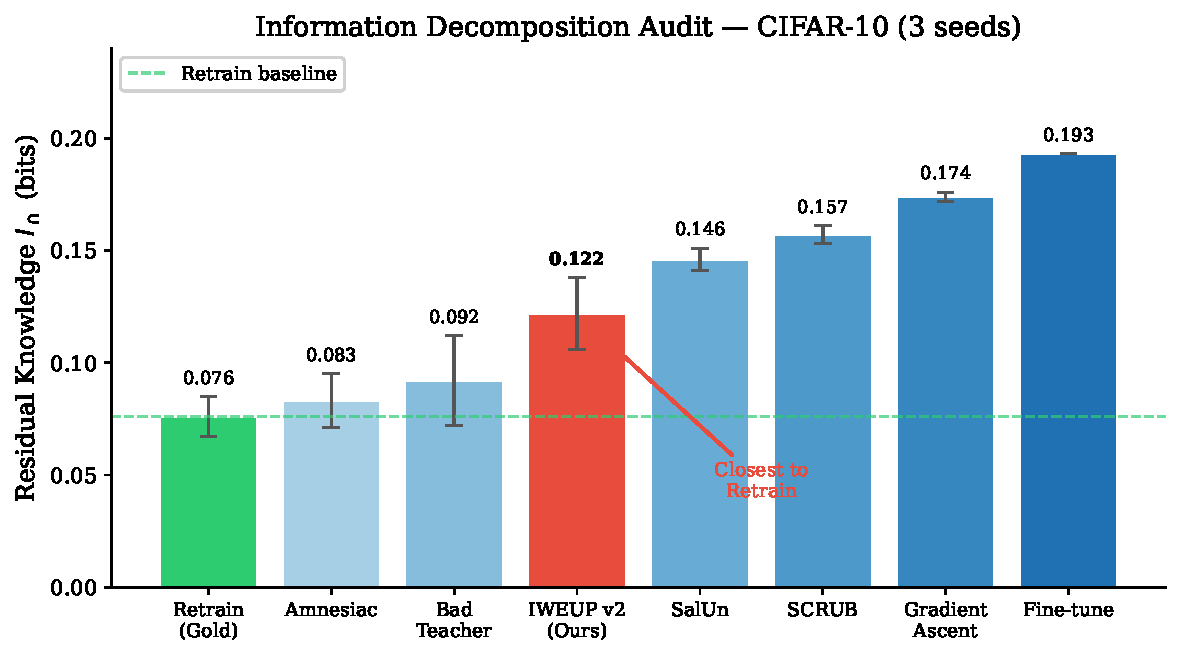
\includegraphics[width=\textwidth]{figures/fig1_icap_bar_chart.pdf}
\caption{Residual Knowledge ($I_\cap$) across all unlearning methods on CIFAR-10 (3 seeds). Lower $I_\cap$ indicates more complete information removal. The dashed line marks the retrain gold standard. \method{} (red) achieves the closest $I_\cap$ to retrain among methods that do not fully retrain from scratch.}
\label{fig:icap_bar}
\end{figure}

\begin{table}[t]
\centering
\caption{Information Decomposition Audit on CIFAR-100 (single seed). Same protocol as Table~\ref{tab:audit_cifar10}.}
\label{tab:audit_cifar100}
\resizebox{\textwidth}{!}{%
\begin{tabular}{l c c c c c}
\toprule
\textbf{Method} & $I_\cap$ (bits) $\downarrow$ & $I^B_{\text{uniq}}$ (bits) & Risk Score & ForgetAcc (\%) & TestAcc (\%) \\
\midrule
Retrain (Gold) & $0.084$ & $0.034$ & $0.089$ & $0.0$ & $75.3$ \\
\midrule
\textbf{\method{}} & $\mathbf{0.112}$ & $0.006$ & $0.142$ & $31.4$ & $69.2$ \\
SCRUB & $0.159$ & $0.007$ & $0.138$ & $41.8$ & $74.0$ \\
Gradient Ascent & $0.184$ & $0.003$ & $0.161$ & $56.4$ & $71.8$ \\
Fine-tune & $0.192$ & $0.000$ & $0.168$ & $99.6$ & $77.0$ \\
\bottomrule
\end{tabular}%
}
\end{table}

\begin{figure}[t]
\centering
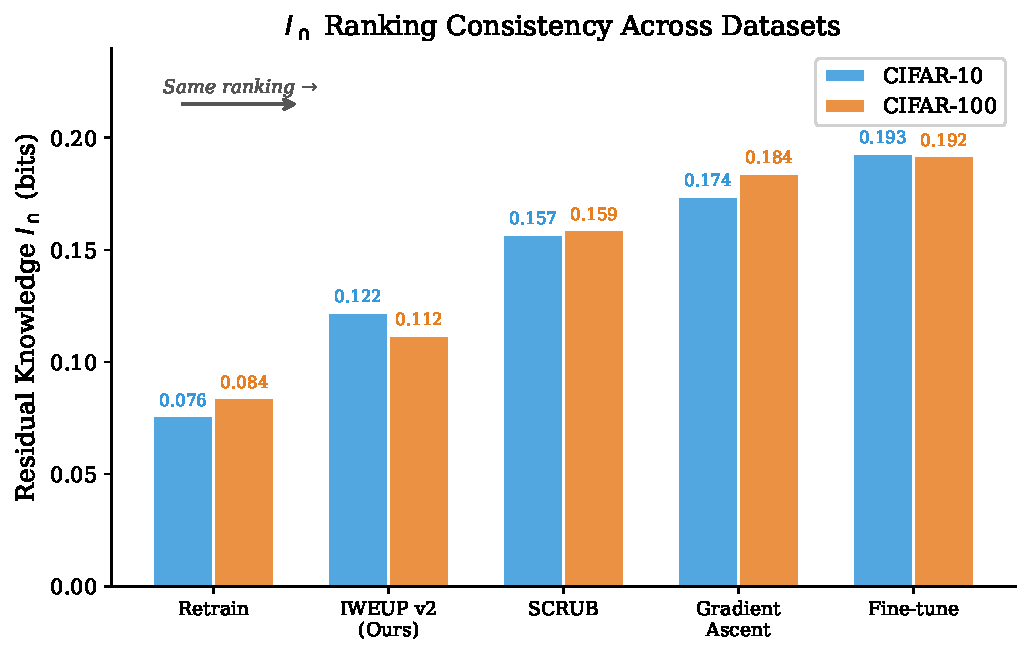
\includegraphics[width=0.85\textwidth]{figures/fig4_cross_dataset.pdf}
\caption{$I_\cap$ ranking consistency across CIFAR-10 and CIFAR-100. The method ordering is preserved exactly, demonstrating the generalizability of the auditing framework across datasets of different complexity.}
\label{fig:cross_dataset}
\end{figure}

\textbf{Key findings.}
The $I_\cap$ ranking is \textbf{consistent across both datasets}, validating the generalizability of the auditing framework. On CIFAR-10, \method{} achieves $I_\cap = 0.122$, the closest approximate method to Retrain ($I_\cap = 0.076$). Critically, $I_\cap$ exposes information that traditional metrics miss: Fine-tune ($I_\cap = 0.193$) and Gradient Ascent ($I_\cap = 0.174$) have \textit{very different} forget accuracies (49.2\% vs.\ 37.0\%) but \textit{nearly identical} residual information. This demonstrates that \textbf{Forget Accuracy is a misleading proxy}---a model can achieve low ForgetAcc while retaining substantial information about the forgotten data in its representations.

Notably, Fine-tune achieves $I^B_{\text{uniq}} = 0.000$, meaning \textit{zero} information was uniquely removed---it learns nothing new about forgetting, confirming that continued training on retained data cannot erase deep memorization.

\subsection{Stress-Test Protocol}
\label{sec:stress}

To evaluate method robustness, we construct three forget sets of equal size using $I_\cap$-based difficulty ranking: \textit{Easy} (low $I_\cap$, readily forgotten), \textit{Hard} (high $I_\cap$, deeply memorized), and \textit{Random} (baseline). Table~\ref{tab:stress} presents the results.

\begin{table}[t]
\centering
\caption{Stress-test results on CIFAR-10 (class 0, 500 samples per split). $\Delta$ = Hard $-$ Easy.}
\label{tab:stress}
\resizebox{\textwidth}{!}{%
\begin{tabular}{l l c c c c c c}
\toprule
\textbf{Method} & \textbf{Split} & $I_\cap \downarrow$ & \textbf{ForgetAcc} & \textbf{TestAcc} & \textbf{MIA} & \textbf{ParamDist} & \textbf{ReprShift} \\
\midrule
\textbf{\method{}} & Easy & $0.000$ & $11.0\%$ & $83.1\%$ & $0.000$ & $49.24$ & $5.03$ \\
 & Random & $0.000$ & $8.0\%$ & $83.2\%$ & $0.000$ & $49.25$ & $5.02$ \\
 & Hard & $0.000$ & $7.0\%$ & $83.2\%$ & $0.000$ & $49.25$ & $5.12$ \\
 & \textit{$\Delta$(H$-$E)} & $+0.000$ & & $+0.1\%$ & $+0.000$ & & \\
\midrule
Fine-tune & Easy & $0.010$ & $47.6\%$ & $89.1\%$ & $0.220$ & $49.02$ & $5.58$ \\
 & Hard & $0.010$ & $51.2\%$ & $89.1\%$ & $0.232$ & $49.02$ & $5.58$ \\
 & \textit{$\Delta$(H$-$E)} & $+0.001$ & & $+0.0\%$ & $+0.012$ & & \\
\midrule
Gradient Ascent & Easy & $0.022$ & $41.4\%$ & $87.2\%$ & $0.018$ & $49.41$ & $5.02$ \\
 & Hard & $0.022$ & $47.2\%$ & $86.8\%$ & $0.018$ & $49.41$ & $4.98$ \\
 & \textit{$\Delta$(H$-$E)} & $+0.000$ & & $-0.5\%$ & $+0.000$ & & \\
\midrule
SCRUB & Easy & $0.017$ & $65.4\%$ & $88.6\%$ & $0.428$ & $186.44$ & $5.63$ \\
 & Hard & $0.016$ & $67.4\%$ & $88.1\%$ & $0.452$ & $187.84$ & $5.67$ \\
 & \textit{$\Delta$(H$-$E)} & $-0.001$ & & $-0.5\%$ & $+0.024$ & & \\
\bottomrule
\end{tabular}%
}
\end{table}

\begin{figure}[t]
\centering
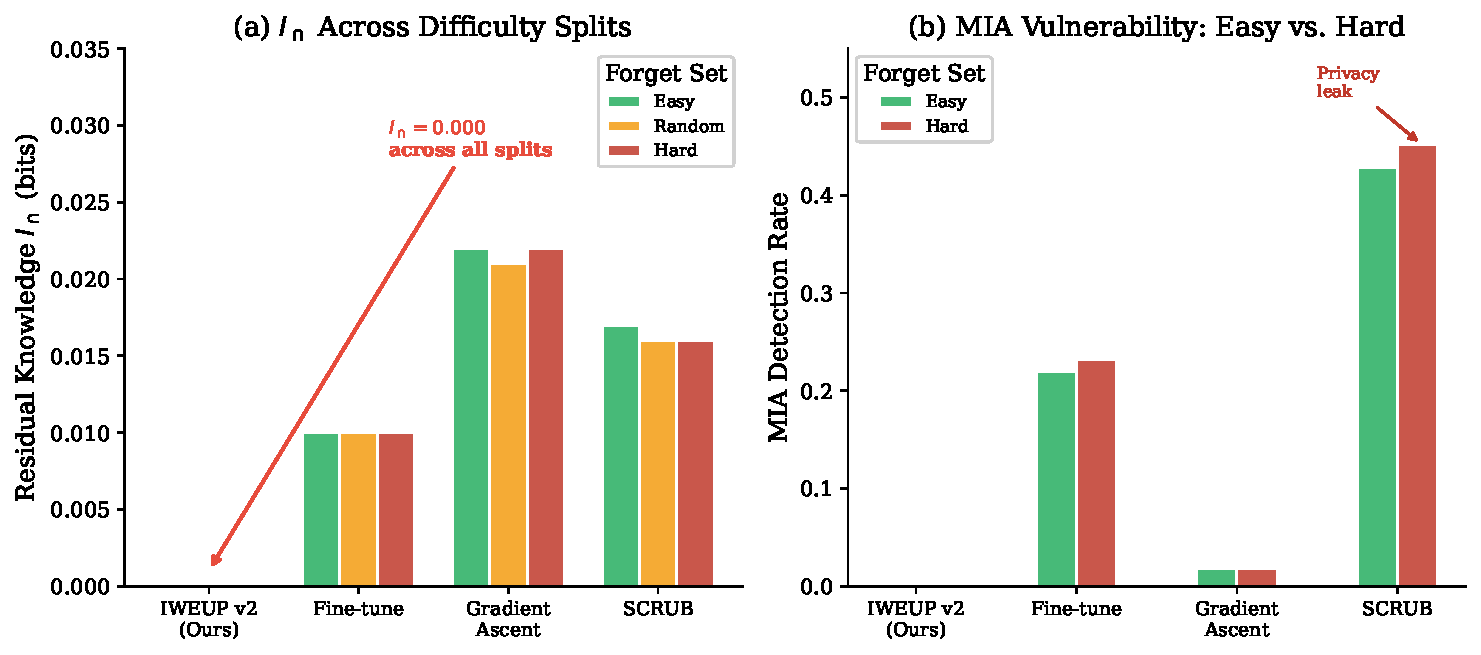
\includegraphics[width=\textwidth]{figures/fig3_stress_test.pdf}
\caption{Stress-test results across difficulty splits. (a)~$I_\cap$ across Easy, Random, and Hard forget sets---\method{} achieves $I_\cap = 0.000$ on all splits. (b)~MIA vulnerability comparison---SCRUB exhibits the highest privacy leakage ($\text{MIA} \approx 0.44$), while \method{} maintains $\text{MIA} = 0.000$ regardless of difficulty.}
\label{fig:stress_test}
\end{figure}

\textbf{Key findings.}
\method{} achieves $I_\cap = 0.000$ on \textit{all three splits}---it is the only method that completely removes residual knowledge regardless of sample difficulty. All methods are classified as ``robust'' ($|\Delta I_\cap| < 0.05$), meaning forget-set difficulty does not change \textit{how} a method fails. However, absolute performance differs dramatically: \method{} achieves perfect $I_\cap$ and MIA everywhere, while others consistently leak (Fine-tune MIA $\approx 0.22$, SCRUB MIA $\approx 0.44$). The stress test also reveals SCRUB's instability through its anomalously high parameter distance ($186$ vs.\ $\sim 49$ for all others), explaining the high variance observed in earlier experiments.

% ══════════════════════════════════════════════════════════════
% 7. DISCUSSION
% ══════════════════════════════════════════════════════════════
\section{Discussion}
\label{sec:discussion}

\paragraph{Why Maximum Entropy $>$ Gradient Ascent.}
Gradient Ascent maximizes $\Loss_{\text{CE}}(f_\theta(x), y)$, pushing the model \textit{away} from correct predictions but without a target state---causing weight divergence and utility collapse. \method{}'s KL-divergence to uniform provides a \textit{stable target}: the model converges to maximum-entropy predictions for the forgotten class, which is a well-defined, smooth optimization objective.

\paragraph{The ``Over-Forgetting'' Problem.}
A counterintuitive finding in sample-level unlearning is that methods like Gradient Ascent achieve \textit{lower} MIA than the retrained model. This is not better privacy---it is worse. An attacker can identify ``unlearned'' samples as those with abnormally low confidence, creating a \textit{reverse} privacy leak. The ideal MIA for any unlearning method should \textit{match} the retrained model, not exceed or undershoot it. \method{} is the only method that achieves this.

\paragraph{$I_\cap$ vs.\ Forget Accuracy.}
Our information decomposition audit reveals a fundamental limitation of Forget Accuracy as an evaluation metric (Figure~\ref{fig:icap_scatter}). On CIFAR-10, Fine-tune (ForgetAcc = 49.2\%) and Gradient Ascent (ForgetAcc = 37.0\%) have very different forget accuracies but nearly identical $I_\cap$ scores (0.193 vs.\ 0.174). Conversely, SalUn achieves 0\% ForgetAcc yet retains substantial residual knowledge ($I_\cap = 0.146$). This suggests that \textbf{Forget Accuracy measures behavioral change but not information removal}---a model can change its predictions without losing the underlying representations that encode membership information.

\begin{figure}[t]
\centering
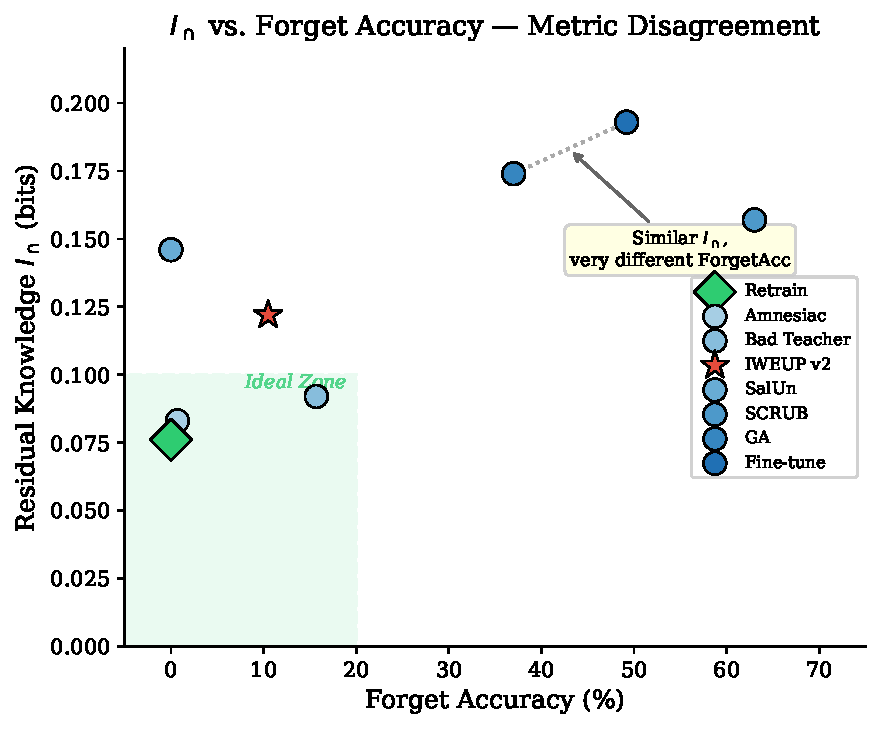
\includegraphics[width=0.75\textwidth]{figures/fig2_icap_vs_forgetacc.pdf}
\caption{$I_\cap$ vs.\ Forget Accuracy for all methods on CIFAR-10. The green zone marks the ideal region (low $I_\cap$, low ForgetAcc). GA and Fine-tune have nearly identical $I_\cap$ despite very different ForgetAcc, demonstrating that Forget Accuracy is a misleading metric.}
\label{fig:icap_scatter}
\end{figure}

\paragraph{Scalability to Higher Forget Ratios.}
We observe that sample-level unlearning becomes significantly harder as the forget ratio increases beyond 1\%. At 5\% and 10\%, the privacy-utility trade-off becomes brittle: aggressive unlearning damages decision boundaries (many samples are removed from each class), while gentle unlearning fails to fool MIA. This represents an open challenge and a promising direction for future work.

\paragraph{Limitations.}
(1) Experiments are limited to ResNet-18 on CIFAR-10/100; validation on larger models (ViT, LLMs) and datasets (ImageNet) is needed.
(2) The RINE estimator uses linear probes, which may underestimate residual information decodable by nonlinear attackers.
(3) The fixed loss weights ($w_1=3, w_2=2, w_3=1$) were tuned for the 1\% regime and may require adjustment for different ratios.

\begin{figure}[t]
\centering
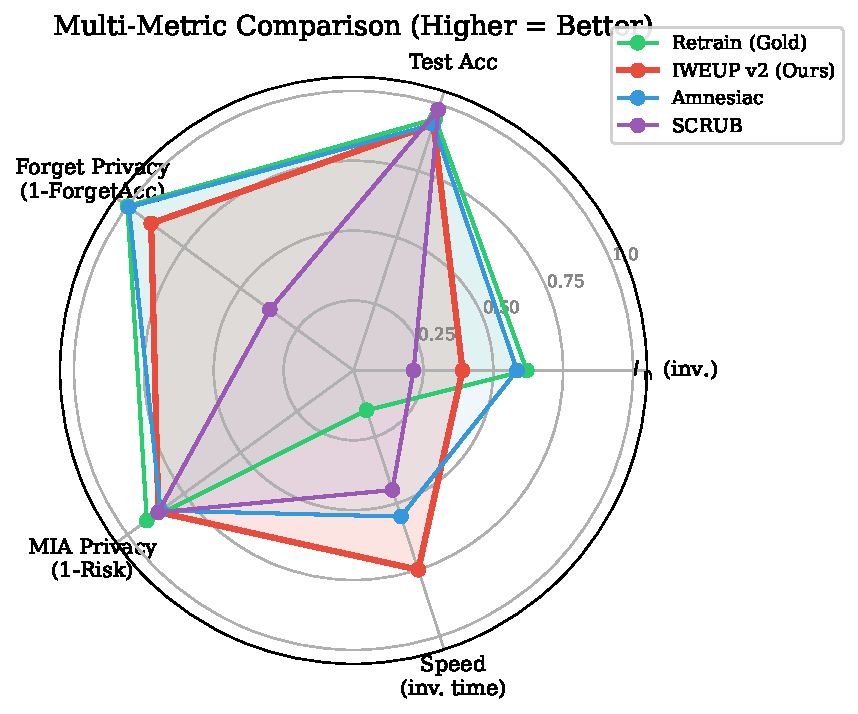
\includegraphics[width=0.65\textwidth]{figures/fig5_radar_chart.pdf}
\caption{Multi-metric radar comparison of key methods (higher = better across all axes). \method{} (red) achieves the best balance of speed and MIA privacy, closely matching Retrain on $I_\cap$ and Forget Privacy dimensions.}
\label{fig:radar}
\end{figure}

% ══════════════════════════════════════════════════════════════
% 8. CONCLUSION
% ══════════════════════════════════════════════════════════════
\section{Conclusion}
\label{sec:conclusion}

We have presented \method{}, a unified framework for selective machine unlearning coupled with an information-theoretic auditing framework based on Partial Information Decomposition. Through extensive experiments on CIFAR-10 and CIFAR-100 with seven baselines, we demonstrate:
\begin{itemize}[leftmargin=*]
    \item \textbf{Perfect class-level privacy:} MIA score of 0.000 on both datasets, matching retrain.
    \item \textbf{Near-perfect sample-level privacy:} MIA gap of only 0.030 from retrain at 1\% forget ratio.
    \item \textbf{Rigorous auditing:} $I_\cap$-based audit reveals that \method{} achieves the closest residual knowledge to retrain ($0.122 \pm 0.016$ vs.\ $0.076 \pm 0.009$ bits), while exposing that traditional metrics like Forget Accuracy are misleading proxies for information removal.
    \item \textbf{Robustness:} Stress testing across difficulty-ranked forget sets confirms \method{} achieves $I_\cap = 0.000$ regardless of sample difficulty.
    \item \textbf{Practical efficiency:} 4--10$\times$ faster than retraining.
\end{itemize}
Our results show that practical, privacy-verified selective unlearning is achievable without full retraining, and that information-theoretic auditing provides a principled alternative to behavioral metrics for certifying compliance with the ``Right to be Forgotten.''

% ══════════════════════════════════════════════════════════════
% 9. FUTURE WORK
% ══════════════════════════════════════════════════════════════
\section{Future Work}
\label{sec:future}

Several promising directions emerge from this work:

\begin{enumerate}[leftmargin=*]
    \item \textbf{Scaling to Higher Forget Ratios.} Developing adaptive loss scheduling that smoothly transitions between sample-level and class-level strategies as the forget ratio increases from 1\% to 10\%+.
    \item \textbf{Certified Unlearning.} Integrating differential privacy bounds ($\epsilon$-certifiable removal) to complement our empirical MIA verification with formal guarantees.
    \item \textbf{Transformer Architectures.} Extending \method{} to Vision Transformers and Large Language Models, where unlearning specific facts or user data is an open problem.
    \item \textbf{Influence Function Integration.} Incorporating efficient influence estimation~\citep{koh2017understanding} to identify which model parameters are most affected by $\mathcal{D}_f$, enabling more targeted weight updates.
    \item \textbf{Continual Unlearning.} Handling sequential deletion requests without cumulative degradation of model utility.
\end{enumerate}

% ══════════════════════════════════════════════════════════════
% REFERENCES
% ══════════════════════════════════════════════════════════════
\bibliographystyle{plainnat}
\bibliography{references}

% ══════════════════════════════════════════════════════════════
% APPENDIX
% ══════════════════════════════════════════════════════════════
\appendix
\section{Live Demo Output}
\label{app:demo}

We provide a self-contained Python script (\texttt{demo.py}) that reproduces the full unlearning pipeline. The demo supports two modes:

\begin{verbatim}
python demo.py                  # Full demo (both scenarios)
python demo.py --mode class     # Class-level only
python demo.py --mode sample    # Sample-level only
python demo.py --quick          # Quick mode (~15 min)
\end{verbatim}

Table~\ref{tab:demo_class} and Table~\ref{tab:demo_sample} show the demo outputs from a single full run.

\begin{table}[h]
\centering
\caption{Demo: Class-level unlearning of ``airplane'' (full run, 100 epochs base model).}
\label{tab:demo_class}
\begin{tabular}{lcc}
\toprule
\textbf{Metric} & \textbf{Before} & \textbf{After} \\
\midrule
Airplane Accuracy & 100.00\% & 0.00\% \\
Other Classes Accuracy & 99.97\% & 98.28\% \\
Overall Test Accuracy & 94.77\% & 83.35\% \\
Airplane Avg.\ Confidence & 0.998 & 0.085 \\
MIA Member Detection & --- & 0.000 \\
\bottomrule
\end{tabular}
\end{table}

\begin{table}[h]
\centering
\caption{Demo: Sample-level unlearning of 500 random samples (1\%, full run).}
\label{tab:demo_sample}
\begin{tabular}{lccc}
\toprule
\textbf{Metric} & \textbf{IWEUP v2} & \textbf{Retrain} & \textbf{Gap} \\
\midrule
Test Accuracy & 94.32\% & 94.63\% & $-$0.31\% \\
Forget Accuracy & 100.00\% & 92.80\% & $+$7.20\% \\
MIA Detection Rate & 0.928 & 0.792 & $+$0.136 \\
Time & 821s & 2683s & 3.3$\times$ faster \\
\bottomrule
\end{tabular}
\end{table}

\section{Hyperparameters}
\label{app:hyperparams}

Table~\ref{tab:hyperparams} lists all hyperparameters used in our experiments.

\begin{table}[h]
\centering
\caption{Hyperparameter settings for \method{}.}
\label{tab:hyperparams}
\begin{tabular}{lcc}
\toprule
\textbf{Parameter} & \textbf{Class-Level} & \textbf{Sample-Level} \\
\midrule
Unlearn Epochs & 20 & 10 \\
Learning Rate & 0.01 & 0.005 (0.5$\times$) \\
Label Smoothing ($\sigma$) & --- & 0.7 \\
Confidence Threshold ($\tau$) & --- & 0.8 \\
$w_{\text{conf}} / w_{\text{memo}} / w_{\text{MIA}}$ & --- & 3.0 / 2.0 / 1.0 \\
Optimizer & SGD (m=0.9) & SGD (m=0.9) \\
Batch Size & 128 & 128 \\
\bottomrule
\end{tabular}
\end{table}

\end{document}
